% Figure from MATH 556 notes, section 17. Compile with the notes preamble.
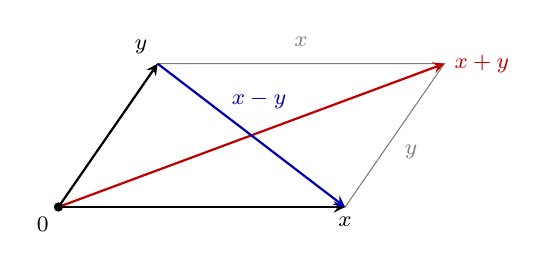
\begin{tikzpicture}[scale=1.4, >=stealth]
\coordinate (O) at (0,0);
\coordinate (X) at (2.6,0);
\coordinate (Y) at (0.9,1.3);
\coordinate (XY) at (3.5,1.3);
\draw[thin, gray] (O) -- (X) -- (XY) -- (Y) -- cycle;
\draw[->, thick] (O) -- (X) node[below, font=\footnotesize] {$x$};
\draw[->, thick] (O) -- (Y) node[above left, font=\footnotesize] {$y$};
\draw[->, thick, red!75!black] (O) -- (XY) node[right, font=\footnotesize] {$x + y$};
\draw[->, thick, blue!70!black] (Y) -- (X) node[pos=0.36, above right, font=\footnotesize, inner sep=2pt] {$x - y$};
\node[font=\footnotesize, gray] at (3.2,0.5) {$y$};
\node[font=\footnotesize, gray] at (2.2,1.5) {$x$};
\fill (O) circle (1.2pt) node[below left, font=\footnotesize] {$0$};
\end{tikzpicture}
